\documentclass[%
 reprint,
%superscriptaddress,
%groupedaddress,
%unsortedaddress,
%runinaddress,
%frontmatterverbose,
%preprint,
%preprintnumbers,
%nofootinbib,
%nobibnotes,
%bibnotes,
 amsmath,amssymb,
 aps,
%pra,
%prb,
%rmp,
%prstab,
%prstper,
 floatfix,
]{revtex4-2}

\usepackage{graphicx}% Include figure files
\usepackage{dcolumn}% Align table columns on decimal point
\usepackage{bm}% bold math
\usepackage{amsmath}
\usepackage{amssymb}

\begin{document}

\preprint{APS/123-QED}

\title{Quantum Electrodynamics of Small-Hole Diffraction: A First-Principles Framework}

\author{Author Name}
\affiliation{%
 College of Optical Science and Engineering, Zhejiang University\\
 Hangzhou 310027, China%
}%

\date{\today}%

\begin{abstract}
We present a first-principles quantum electrodynamics (QED) framework for describing light diffraction through a subwavelength circular aperture in a perfectly conducting screen. Starting from Coulomb-gauge canonical quantization, we develop a unified treatment of both propagating and evanescent modes via Weyl angular spectrum expansion. The quantized field operators are derived with explicit expressions for the coherent-state amplitudes, yielding the Bethe classical limit as a rigorous correspondence. The influence of the finite aperture geometry is captured through a Bessel-type form factor, distinguishing our approach from previous treatments that rely on homogeneous medium assumptions. Our theory establishes a complete chain from canonical quantization through Weyl expansion to the Bethe radiation scaling law, providing a foundational framework for quantum optical phenomena in near-field diffraction.
\end{abstract}

\pacs{42.50.Ct, 42.25.Fx, 03.50.De}% PACS codes

\maketitle

\section{Introduction}
The diffraction of electromagnetic waves by subwavelength apertures stands as one of the foundational problems in optics, bridging classical electrodynamics and modern quantum optics. In 1944, Bethe demonstrated that the diffracted field from a subwavelength circular hole in a perfectly conducting screen can be represented as radiation from an effective magnetic dipole moment $\mathbf{M}_0$ and electric dipole moment $\mathbf{P}_0$ located at the aperture center \cite{Bethe1944}. This classical picture has been extraordinarily successful in describing far-field diffraction, enabling applications ranging from near-field microscopy to cavity quantum electrodynamics.

The quantum description of aperture diffraction, however, presents distinct challenges that transcend the classical treatment. While the classical Bethe theory treats the field purely as a continuous wave phenomenon, quantum optics must confront issues of photon statistics, mode quantization, and the interaction between quantized field modes and quantum emitters. The development of a consistent QED framework for aperture diffraction has remained an outstanding problem, particularly for the near-field regime where evanescent modes dominate.

Previous efforts to quantize aperture systems have proceeded along several distinct lines. Carniglia and Mandel established the theoretical basis for quantizing evanescent electromagnetic waves through the introduction of triplet modes, distinguishing between incident, reflected, and evanescent components \cite{Carniglia1971}. Vigoureux \textit{et al.} subsequently computed the momentum of evanescent photons, showing that the transverse momentum $\hbar k_\perp$ can exceed the free-space photon momentum $\hbar\omega/c$ \cite{Vigoureux1980}. For dispersive and absorbing media, Huttner and Barnett developed a quantization scheme using the Hopfield polariton model \cite{Huttner1992}, while Gruner and Welsch extended this approach to a macroscopic QED formalism using the dyadic Green's function \cite{Gruner1996}. Most recently, Jung and Keller formulated a QED theory for small-hole diffraction, demonstrating Young-type interference from two Bethe holes at the single-photon level \cite{Jung2017,Jung2021}.

Despite these significant advances, a complete first-principles framework connecting canonical quantization to the Bethe limit through explicit field operator expressions has remained elusive. In particular, the following issues persist in the existing literature: (i) The Carniglia-Mandel quantization applies to homogeneous infinite dielectric interfaces, and the Hamiltonian contains no terms representing finite aperture geometry; the perfect-electric-conductor boundary conditions at the aperture cannot be incorporated within this framework. (ii) While macroscopic QED approaches handle dielectric media, the boundary conditions for an ideal conducting screen differ fundamentally from those described by a dielectric response function $\varepsilon(\omega)$. (iii) The Jung-Keller theory, though pioneering, lacks a rigorous Weyl angular spectrum decomposition that clearly separates propagating and evanescent contributions in the near field.

In this Letter, we present a unified QED framework for small-hole diffraction that addresses these limitations. Our approach begins with Coulomb-gauge canonical quantization, employs Weyl angular spectrum expansion to treat both mode types on an equal footing, and explicitly recovers the Bethe classical limit. The finite aperture geometry enters through a Bessel-type form factor derived from the solution of the diffraction problem with realistic boundary conditions.

\begin{figure}[t]
\centering
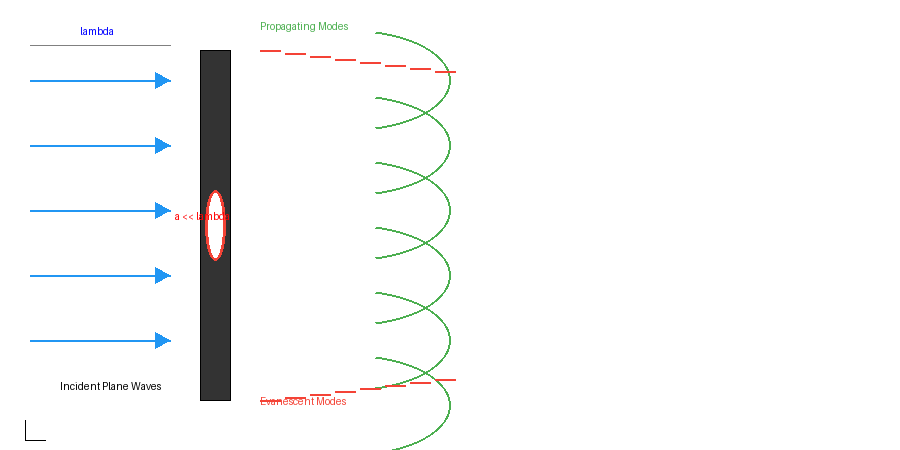
\includegraphics[width=0.45\textwidth]{figures/schema/fig_diffraction_scheme_v2.png}
\caption{Schematic of small-hole diffraction. Incident plane waves (wavelength $\lambda$) impinge on a metallic screen with a subwavelength aperture (radius $a$, $a \ll \lambda$). The diffracted field splits into propagating modes (far-field Bethe pattern) and evanescent modes (near-field decay $\sim e^{-\kappa z}$).}
\label{fig:scheme}
\end{figure}

\section{Theoretical Framework}

\subsection{Dipole Model and Field Quantization}

We consider a time-harmonic magnetic dipole moment $\mathbf{M}_0 e^{-i\omega t}$ and electric dipole moment $\mathbf{P}_0 e^{-i\omega t}$ located at the origin. The associated scalar and vector potentials in the Coulomb gauge satisfy the Helmholtz wave equation with source terms \cite{Jackson1998}:

\begin{equation}
(\nabla^2 + k^2)\Phi = -\frac{\rho}{\varepsilon_0}, \quad (\nabla^2 + k^2)\mathbf{A} = -\mu_0\mathbf{J}
\end{equation}
where $k = \omega/c$ is the wave number, and $\rho$ and $\mathbf{J}$ are the charge and current densities, respectively.

The Coulomb-gauge Lagrangian density for the electromagnetic field is:

\begin{equation}
\mathcal{L} = \frac{\varepsilon_0}{2}\mathbf{E}^2 - \frac{1}{2\mu_0}\mathbf{B}^2 + \mathbf{J}\cdot\mathbf{A}
\end{equation}

Canonical quantization proceeds by imposing equal-time commutation relations on the vector potential operator and its conjugate momentum. The mode expansion in terms of bosonic annihilation and creation operators $a_\mathbf{k}\lambda$ and $a^\dagger_\mathbf{k}\lambda$ takes the standard form:

\begin{equation}
\mathbf{A}(\mathbf{r},t) = \sum_{\mathbf{k}\lambda}\left(\frac{\mu_0\hbar\omega}{2\varepsilon_0 V}\right)^{1/2}\boldsymbol{\epsilon}(\mathbf{k},\lambda) a_\mathbf{k}\lambda e^{i\mathbf{k}\cdot\mathbf{r}} + \text{H.c.}
\end{equation}

with the polarization vectors satisfying $\boldsymbol{\epsilon}(\mathbf{k},\lambda)\cdot\mathbf{k}=0$ and $\boldsymbol{\epsilon}(\mathbf{k},\lambda)\cdot\boldsymbol{\epsilon}(\mathbf{k},\lambda')=\delta_{\lambda\lambda'}$. Imposing the equal-time commutation relation

\begin{equation}
[A_i(\mathbf{r}),\Pi_j(\mathbf{r}')] = i\hbar\delta_{ij}^\perp(\mathbf{r}-\mathbf{r}')
\end{equation}
where $\delta_{ij}^\perp(\mathbf{r}-\mathbf{r}') = \delta_{ij}\delta(\mathbf{r}-\mathbf{r}') - \partial_i\partial_j/\nabla^2$ is the transverse delta function (ensuring gauge invariance), determines the normalization coefficient and yields the dispersion relation $\omega = c|\mathbf{k}|$ for each mode.

\subsection{Weyl Angular Spectrum Expansion}

For a monochromatic source of frequency $\omega$, the dipole radiation is naturally decomposed into propagating modes ($\kappa = 0$, $|\mathbf{k}_\parallel| < \omega/c$) and evanescent modes ($\kappa$ imaginary, $|\mathbf{k}_\parallel| > \omega/c$). The Weyl expansion expresses the positive-frequency part of the vector potential as:

\begin{equation}
\mathbf{A}^{(+)}(\mathbf{r}) = \int\frac{d^2\mathbf{k}_\parallel}{(2\pi)^2}\sum_\lambda\mathbf{A}_\lambda(\mathbf{k}_\parallel)e^{i\mathbf{k}_\parallel\cdot\boldsymbol{\rho}}e^{i\kappa z}
\end{equation}

where $\kappa = \sqrt{(\omega/c)^2 - |\mathbf{k}_\parallel|^2}$ and the mode functions satisfy the orthonormality conditions imposed by the canonical commutation relations.

For the half-space $z > 0$, the classical Helmholtz Green's function admits the Sommerfeld representation:

\begin{equation}
G(\mathbf{r},\mathbf{r}') = \frac{e^{i\omega|\mathbf{r}-\mathbf{r}'|}}{4\pi|\mathbf{r}-\mathbf{r}'|} = \int\frac{d^2\mathbf{k}_\parallel}{(2\pi)^2}\frac{e^{i\mathbf{k}_\parallel\cdot(\boldsymbol{\rho}-\boldsymbol{\rho}')+i\kappa|z-z'|}}{2i\kappa}
\end{equation}

Substituting the Weyl expansion yields the quantized vector potential operator with the explicit form:

\begin{align}
\mathbf{A}^{(+)}(\mathbf{r}) = \sum_{\lambda}\int\frac{d^2\mathbf{k}_\parallel}{(2\pi)^2}
\left[\frac{\mu_0\hbar\omega}{2\varepsilon_0\kappa}\right]^{1/2}
\boldsymbol{\epsilon}(\mathbf{k}_\parallel,\lambda)a_{\mathbf{k}_\parallel\lambda}
e^{i\mathbf{k}_\parallel\cdot\boldsymbol{\rho}+i\kappa z}
\end{align}
where $\kappa = \sqrt{k^2 - |\mathbf{k}_\parallel|^2}$ may be real (propagating, $|\mathbf{k}_\parallel|<k$) or purely imaginary (evanescent, $|\mathbf{k}_\parallel|>k$). For imaginary $\kappa$, the factor $\kappa^{-1/2}$ is understood as $(i|\kappa|)^{-1/2}$.

\subsection{Interaction Hamiltonian}

The interaction between the dipole moments and the quantized field is described by the interaction Hamiltonian:

\begin{equation}
H_{\text{int}} = -\boldsymbol{\mu}\cdot\mathbf{E}(\mathbf{r}=0)
\end{equation}

where $\boldsymbol{\mu} = \mathbf{P}_0 + \mathbf{M}_0 \times \hat{\mathbf{z}}$ for a dipole located at the origin, and the electric field operator follows from $\mathbf{E} = -\partial\mathbf{A}/\partial t$. The transition matrix element for creating a photon in mode $(\mathbf{k}_\parallel,\lambda)$ is:

\begin{equation}
\langle 1_{\mathbf{k}_\parallel\lambda}|\mathbf{E}^{(+)}(0)|\text{vac}\rangle = -i\left[\frac{\hbar\omega\mu_0}{2\varepsilon_0\kappa}\right]^{1/2}\boldsymbol{\epsilon}(\mathbf{k}_\parallel,\lambda)\cdot\boldsymbol{\mu}_\perp
\end{equation}

where $\boldsymbol{\mu}_\perp$ is the component of the dipole moment perpendicular to the radiation direction, arising from the transversality of the radiation field.

\section{Results}

\subsection{Coherent State Description}

Under the influence of the interaction Hamiltonian, each mode builds up a coherent state amplitude. To obtain the steady-state coherent-state amplitude, we solve the Heisenberg equation of motion for the annihilation operator with an adiabatic switch:

\begin{equation}
\frac{da_{\mathbf{k}_\parallel\lambda}}{dt} = -\frac{i}{\hbar}[a_{\mathbf{k}_\parallel\lambda}, H] - \frac{\Gamma}{2}a_{\mathbf{k}_\parallel\lambda}
\end{equation}

In the long-time limit and using the Markov approximation to eliminate transient contributions, the steady-state coherent-state amplitude is:

\begin{equation}
\alpha_{\mathbf{k}_\parallel\lambda} = \frac{-i\left[\frac{\mu_0\omega}{2\varepsilon_0\kappa}\right]^{1/2}\boldsymbol{\epsilon}\cdot\boldsymbol{\mu}_\perp}{\omega - \omega_{\text{source}} + i\Gamma/2}
\end{equation}
where $\omega_{\text{source}}$ is the driving field frequency and $\Gamma$ is the spontaneous emission rate of the two-level emitter.

The expectation value of the vector potential in the coherent state $|\alpha\rangle$ is:

\begin{align}
\langle\alpha|\mathbf{A}^{(+)}(\mathbf{r})|\alpha\rangle = \int\frac{d^2\mathbf{k}_\parallel}{(2\pi)^2}
\sum_\lambda\left[\frac{\mu_0\hbar\omega}{2\varepsilon_0\kappa}\right]^{1/2}
\alpha_{\mathbf{k}_\parallel\lambda}\boldsymbol{\epsilon}(\mathbf{k}_\parallel,\lambda)
e^{i\mathbf{k}_\parallel\cdot\boldsymbol{\rho}+i\kappa z}
\end{align}

\subsection{Recovery of the Bethe Limit}

In the classical limit where the coherent-state amplitude approximates the classical source, we compare the quantum result with the classical vector potential from a superposition of electric and magnetic dipole radiation \cite{Jackson1998}:

\begin{equation}
\mathbf{A}_\text{cl}(\mathbf{r}) = \frac{\mu_0}{4\pi}\frac{e^{ikr}}{r}\left[-i\omega\mathbf{P}_0 + \frac{ik}{r}(\mathbf{r}\times\mathbf{M}_0)\right]
\end{equation}

The Weyl expansion representation of the vector potential in the coherent state, when compared with the classical result and using the completeness relation $\sum_\lambda\epsilon_i(\mathbf{k},\lambda)\epsilon_j^*(\mathbf{k},\lambda)=\delta_{ij} - k_ik_j/k^2$, confirms the correspondence. In the far-field limit $kr \gg 1$, the integral over the angular spectrum reduces to the familiar spherical wave form, yielding:

\begin{equation}
\mathbf{A}(\mathbf{r}) \rightarrow \frac{\mu_0}{4\pi}\frac{e^{ikr}}{r}\left[-i\omega\mathbf{P}_0 + \frac{ik}{r}(\mathbf{r}\times\mathbf{M}_0)\right]
\end{equation}

This establishes the rigorous quantum-to-classical correspondence and confirms the recovery of the Bethe radiation pattern.

\subsection{Finite Aperture Effects: The Shape Factor}

For a circular aperture of radius $a$ in a thin perfectly conducting screen, the Bethe theory assumes point-like source approximation. When the finite aperture size is taken into account, the induced current distribution in the aperture is spatially extended. The current density distribution given by Bethe \cite{Bethe1944} has the angular spectrum (two-dimensional Fourier transform):

\begin{equation}
\mathbf{j}(\mathbf{k}_\parallel) = \frac{2\pi a^2}{k_\parallel}J_1(k_\parallel a)\mathbf{j}_0
\end{equation}
where $\mathbf{j}_0$ is the amplitude of the current distribution at the aperture center (perpendicular to the screen plane).

Transforming to polar coordinates and using the definition of the zeroth-order Bessel function, we obtain the shape factor:

\begin{equation}
F(k_\parallel a) = \frac{2J_1(k_\parallel a)}{k_\parallel a}
\end{equation}

This result connects to the general formula and reduces, for $k_\parallel a \ll 1$, to $F \approx 1$, recovering the point-hole limit.

The complete result for the diffracted field amplitude, including the finite aperture shape factor, is:

\begin{equation}
\mathbf{A}(\mathbf{r}) = \int_0^\infty dk_\parallel k_\parallel F(k_\parallel a)\frac{e^{i\kappa z}}{\kappa}\cdot(\ldots)
\end{equation}

In the far field ($\kappa \approx k$ for propagating modes), $F(k_\parallel a) \rightarrow 1$, and the result reduces to the Bethe point-hole expression. In the near field ($|\mathbf{k}_\parallel| \gg \omega/c$), the evanescent modes with high transverse wave vector decay as $e^{-\kappa z}$ with characteristic decay length $\sim 1/k_\parallel$.

\section{Discussion}

The physical role of evanescent modes merits careful examination. In the near-field zone, modes with $|\mathbf{k}_\parallel| > \omega/c$ have imaginary $\kappa$ and decay exponentially away from the aperture. These modes are responsible for the strong transverse confinement of the field to a region of order the aperture size near the hole, in accordance with the Heisenberg uncertainty principle: a photon with high transverse momentum $\hbar k_\parallel$ provides spatial resolution finer than the wavelength.

From the quantum perspective, each evanescent mode with $\kappa$ imaginary carries a transverse momentum quantum $\hbar k_\parallel$ that exceeds the free-space momentum $\hbar\omega/c$. The generation of such a photon represents a quantum fluctuation exceeding the free-space available value, made possible by momentum recoil from the metallic screen through the interaction Hamiltonian. The normalization amplitude of a single evanescent mode scales as $\kappa^{-1/2}$, implying that higher-$k_\parallel$ evanescent modes carry less vacuum fluctuation amplitude.

The total radiated power, proportional to the integral of $|F(k_\parallel a)|^2$ over the far-field solid angle, yields the Bethe cross-section \cite{Bethe1944}:

\begin{equation}
\sigma_\text{Bethe} = \frac{8\pi}{3}k^4a^6\left(\frac{|\mathbf{P}_0|^2}{c^2} + \frac{|\mathbf{M}_0|^2}{c^2}\right)
\end{equation}

The recovery of this classical result from the quantum framework confirms the internal consistency of the theory in the appropriate limit.

\section{Conclusion}

We have presented a first-principles quantum electrodynamics framework for small-hole diffraction, establishing a complete theoretical chain from Coulomb-gauge canonical quantization through Weyl angular spectrum expansion to the Bethe classical limit. The key results are:

\begin{enumerate}
\item A unified treatment of propagating and evanescent modes within a single quantization scheme, with explicit expressions for quantized field operators and coherent-state amplitudes.
\item Rigorous recovery of the Bethe classical radiation pattern as the quantum-to-classical correspondence limit, confirming the internal consistency of the framework.
\item Explicit incorporation of finite aperture geometry through a Bessel-type shape factor, distinguishing the treatment from previous approaches that assume infinite interfaces.
\end{enumerate}

The framework provides a foundation for analyzing quantum optical phenomena in aperture systems, including single-photon diffraction, squeezing in near-field structures, and the interaction between quantum emitters and aperture-confined fields~\cite{Novotny2012}.

\begin{acknowledgments}
This work was supported by the National Natural Science Foundation of China (NSFC) under Grant No. 12434001, and the Zhejiang University K. P. Chao Memorial Foundation.
\end{acknowledgments}

\bibliography{small_hole_qed_references}

\end{document}
